\chapter{Conclusion}

What, then, has our body of work, as well as the numerous other recent investigations into mergers, their remnants, and post-merger evolution, taught us about the fate of sub-\Mch\ CO WD mergers?  Are there mergers that follow the \citeal{vkercj10} scenario of compressing and heating enough during post-merger evolution to ignite degenerate carbon burning near their centers, and then experiencing nuclear simmering until they explode?  Below, I summarize our current understanding of these systems and the \citeal{vkercj10} scenario, and suggest avenues for future exploration.

\section{Mergers and Early Post-Merger Evolution}

In Ch. \ref{ch:ch2}, we used 3D SPH simulations of double CO WD mergers to explore the range of possible merger remnants to determine which among them are candidates for ignition during post-merger evolution.  The properties most important for post-merger near-central ignition are the temperature and degree of rotational support of the dense remnant core, and we find that dissimilar-mass mergers feature cold, slowly rotating and degeneracy support cores, while similar-mass ones have hotter cores that are partly rotationally supported.  The (rough) dividing line between the two classes is a density ratio between donor and accretor WD of $\qrho\simeq0.6$, equivalently a difference between their masses of $\Delta M \simeq 0.1\,\Msun$.

Since the publication of Ch. \ref{ch:ch2} as \cite{zhu+13}, \cite{dan+14} published their extensive study of remnants from synchronized WD mergers with exact initial conditions.\footnote{Their remnant profiles are available at \url{http://www.hs.uni-hamburg.de/DE/Ins/Per/Dan/wdwd_remnants}.}  They find for all of their merger remnants, even those we deem similar-mass, that the mass enclosed within the radius of maximum temperature is approximately the mass of the accreting WD (i.e. $\MencTmax\simeq\Ma$), and the temperature at the center is a factor of at least a few lower.  Their similar-mass mergers also do not substantially mix, as ours do.  \cite{dan+14} link these differences to their use of synchronized and exact initial conditions -- indeed, their approximate and unsynchronized merger remnants resemble ours -- which is consistent with our findings in Sec. \ref{sec:c2_variation} that synchronization and longer periods of mass-transfer prior to coalescence make merger remnants more dissimilar-looking.

In Ch. \ref{ch:ch3} we compared a similar-mass $0.625-0.65\,\Msun$ merger simulated in SPH with one in the moving mesh code \arepo.  The two simulations produce very similar results, including for the degree of mixing between the two stars, up to coalescence.  Following coalescence, however, the \arepo\ remnant retains a dense core that is a factor of $\sim2$ colder than its surroundings until the end of the simulation.

Taken together, these results raise the question of whether \textit{any} merger remnants have dense cores substantially heated by the merger, or if our results from Ch. \ref{ch:ch2} depend upon on the hydrodynamic scheme being used, the accuracy of the simulation's initial conditions and the synchronization of the WDs.  A resolution to this issue will require further investigation.  The influence of the hydrodynamic scheme will likely be pinned down once the features that make \gasoline\ and \arepo\ differ are found out, where we ca simulate using \gasoline 2 with the upcoming Eulerian grid simulations by \cite{katz+16} perhaps able to help as well.  The equilibrium solution for a non-rotating close binary is known \citep{uryue98}, and we have made preliminary attempts to implement it into \gasoline.  Resolution of the synchronization debate will come with a better understanding of the influence of tides in WD binaries, perhaps through observationally {\charles MARTEN?}.

Further complicating matters is the dramatic amplification of initially insignificant magnetic fields discussed in Ch. \ref{ch:ch4}, which, through (potentially non-local) dissipation of differential rotation, could serve as an alternate source of heat for the remnant core.  We have already noted potential issues with our results stemming from our use of the Powell divergence cleaner in Sec. \ref{sec:c4_postscript}, but we also note that the remnant field configuration will depend on mixing.  Ch. \ref{ch:ch2} and \citep{dan+14} note that in synchronized mergers contact between the accretion stream and accretor is less violent, and results in a less severe shear layer -- this could reduce the overall growth of the magnetic field.  Moreover, during the merger the field is advected into the system's center of mass, which causes the remnant core to be highly magnetized.  This might not happen in a dissimilar mass merger.  Many of these uncertainties can be eliminated by running \arepo\ mergers using the new constrained transport module for both synchronized and non-synchronized WD binaries.

Ch. \ref{ch:ch3} also showed the onset of an $m = 1$ spiral mode due to gravitational perturbation of the disk by the non-axisymmetric remnant core.  This spiral mode hydrodynamically transports the angular momentum outward on a timescale a factor of a few faster than estimates of the magnetically-mediated viscous evolution. Since travelling waves can be non-dissipational, the heating resulting from this wave transport may be different than if the trnasport was mediated by viscosity.  The MHD simulation of Ch. \ref{ch:ch4}, however, shows the remnant core becoming axisymmetry $\sim300\,\mrm{s}$ after coalescence, likely as a result of the magnetic field acting upon differential rotation.  Therefore, the lifetime of this wave transport will also depend on how long the non-axisymmetry will last.

(Fig. \ref{fig:c2_deltamcomp})

We note that the modifications discussed above all make it less likely for the remnant core to be heated, spun-up or highly magnetized.  Thus, our merger remnants in Ch. \ref{ch:ch2} are probably upper limits.

Mergers

%- no longer get really hot in their centres.  The older simulations that vk10 based their ideas off of assumed approximate and irrotational mergers with large artificial viscosities.  Our SPH scheme gives similar (if somewhat cooler (Sec compare with Loreig) results), but other codes that are synchronized and use accurate initial conditions do not (check raskin+12 and dan+14 profiles?)  In particular, dan compares their simulations to ours, and find that their similar mass mergers mix less and (consequently) are hottest at their surfaces.

%- while the arepo simulations are quite similar to the gasoline ones, this is the big difference between our two simulations: the 0.625-0.65 Msun merger in Gasoline is evenly heated, while the dense core is in Arepo is not, and remains much colder.  In the case of a purely hydrodynamic evolution even in Arepo there's no obvious way to heat the core other than adiabatic compression.  the core no longer mixes during this phase, so there's no way of bringing hot gas to the deep interior of the core.

- this leaves two problems:
	- is central ignition no longer possible?  perhaps not - synchronized mergers don't do it, and dan notes that his mergers are at least partly unsynchronized by the time they merge.
	- if not, how off center will any ignition occur?  This is difficult to say, and unfortunately depends both on the initial conditions of the WD 
	- thus, our mergers are likely 

-jI+13 non-local heating through magnetic reconnection?  compression looks mostly to be adiabatic, except near the very end (though they do see a trend of INCREASING temperature toward the center with resolution)

- can we rule out the possibility of the standard Yoon et al. model?  No.

\section{Simmering and Explosions}

In Ch. \ref{ch:ch5} we investigated the evolution of sub-\Mch\ WDs that initialize center-lit nuclear fusion, looking in particular for the minimum mass \Mcrit\ of a CO WD that achieves dynamical burning and explodes, rather than expanding and cooling.  We find this mass to be $1.135\,\Msun$, which changes by less than $\sim0.01\,\Msun$ if the WD possesses sub-critical solid-body rotation.  

and $\sim0.02\,\Msun$, respectively.

.  We also estimate that including rotation or $\lesssim 10^{11}\,\mrm{G}$ magnetic fields alters this value by less than $\sim0.01\,\Msun$ and $\sim0.02\,\Msun$, respectively.  Stronger, $\sim10^{12}\,\mrm{G}$ fields, which may be generated through convective dynamo processes, could affect simmering much more substantially, but are beyond the scope of our models.  Examining merger remnants in \citeal{zhu+13}, and the simulation of \cite{ji+13}, we estimate that the majority of sub-\Mch\ post-viscous remnants are too underdense to remain degenerate until dynamical burning if simmering were to set in.  Even if they could explode, they would still produce very little \Ni.  This presents an issue for to the viability of the \citeal{vkercj10} channel, as it suggests most sub-\Mch\ remnants do not explode as SNe Ia.

% We also find that simmering is well-described by approximating the convective zone's temperature profile as adiabatic, with $\Mcrit$ changing by just $\sim0.01\,\Msun$ compared to more accurate models.  and we stress the merit of further study

Ours is a first-order estimate of the simmering process.  Aside from the clear need for more advanced prescriptions of magnetoconvection, future models would also benefit from including eg. modifications to the convective velocity structure resulting from heating or work to expand the WD as it becomes non-degenerate (\citeal{piroc08}, though their effects will primarily be felt far from center of the WD).  A more accurate analysis of the simmering of post-viscous merger remnants could be made by directly using their simulated density, temperature and rotation profiles as initial conditions.  We also use the analytic 1D criterion of \citeal{wooswk04} to determine the end of simmering, and better estimates can be made by taking into account the range of temperatures and velocities of individual convective flows.  This has already been done for \Mch\ WDs using 3D hydrodynamic simulations \citep{kuhlwg06, zing+09, zing+11, nona+12}, which could be extended to lower-mass WDs.

% Zing+09 Fig. 9, 10, gives ignition at slightly lower temperature of 7e8 K.  Zing+11 Fig. 6 gives similar value, as does Nona+12 Fig. 3

We have also estimated the \Mtot-\MNi\ relationship of simmering sub-\Mch\ WDs that reach explosion and find that they, like many other models, do not correspond to the observed SN Ia \Mtot-\MNi\ relationships of \cite{scalzrs14} and \cite{chil+15}.  In particular, our most massive WDs produce too much \Ni\ to reproduce the bottom right of Fig. \ref{fig:mni}, which would not be the case if the temperature structure at the end of simmering were substantially shallower than in our models.  Such a structure could potentially be produced if the burning were not center-lit, but occurred in an off-center shell that remained degenerate throughout the runaway, and we explore this possibility in the companion paper to this work (Heringer et al. in preparation).


How off-center can simmering be?

\begin{figure}
\centering
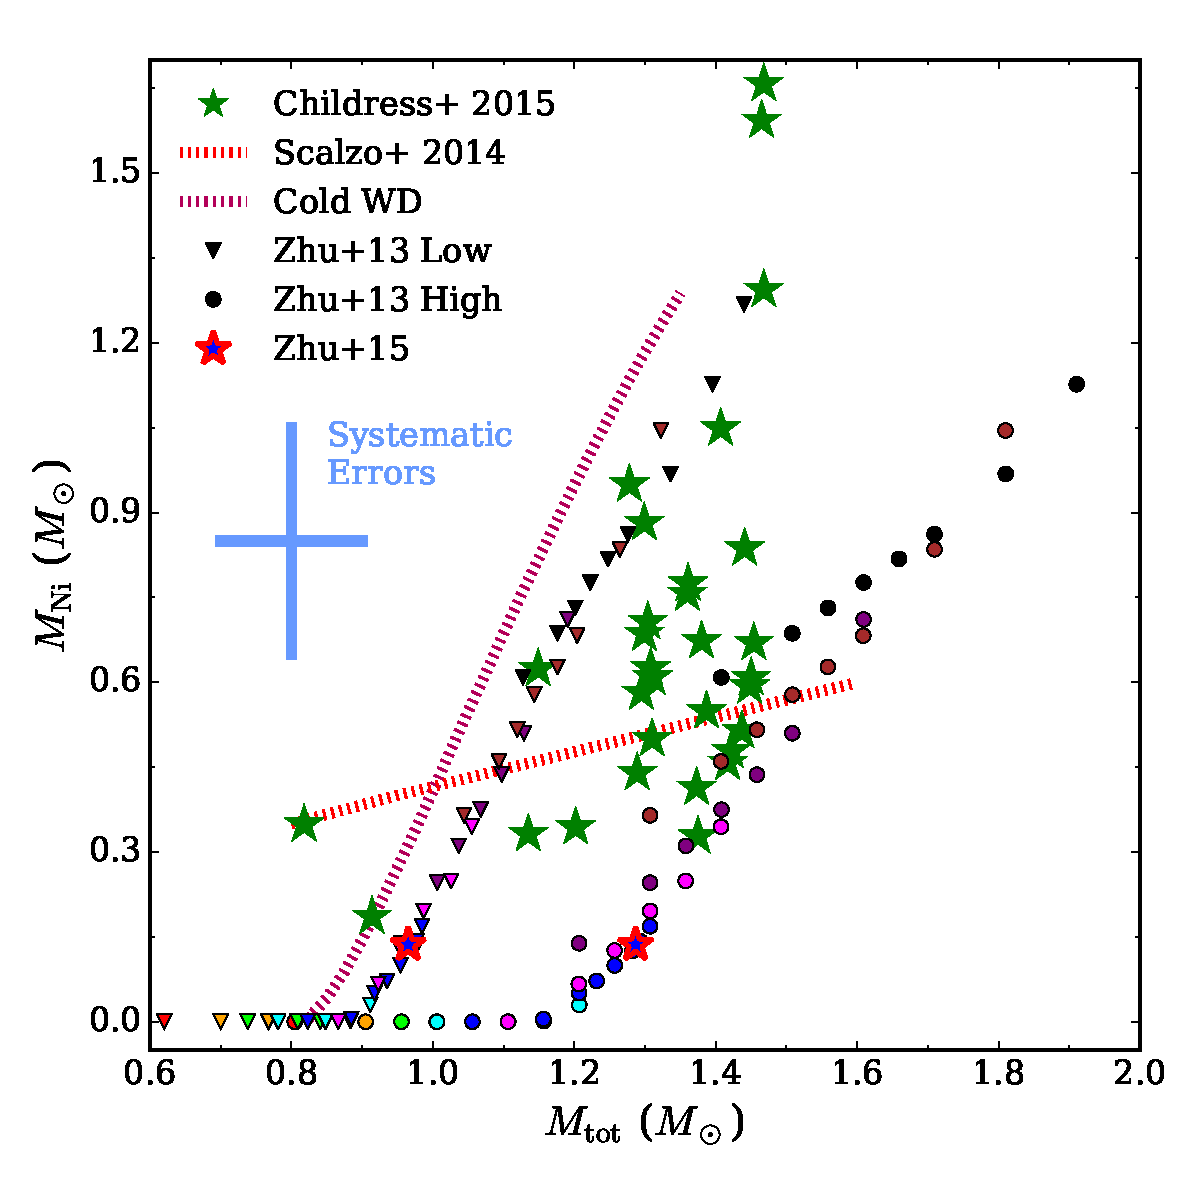
\includegraphics[angle=0,width=0.6\columnwidth]{conclusion/figures/c_MNi.pdf}
\caption{Relationships between total ejected mass \Mtot\ and synthesized \Ni\ mass \MNi\ for adiabatic and \dnabconv-inclusive WDs that experience a pure detonation immediately after the end of simmering, estimated using \cite{sim+10}.  Also plotted are the \Mtot\ and \MNi\ yields of $31$ observed SNe Ia from \cite{chil+15}, and the relationship derived by \cite{scalzrs14} from 337 observed SNe Ia.  \cite{chil+15}'s systematic error bars, indicating how much their values can be shifted in unison, are also included.  The dashed magenta line is the relationship for the pure detonation of cold (uniform $10^5$ K) WDs, with the simulation results of \cite{sim+10} overdrawn.}
\label{fig:c_mcmce_mni}
\end{figure}

\section{Observational Avenues of Exploration}

Finally, we stress the importance of observational work in this field.  Recently revealed properties of the hot DQ population tantalizingly suggest they represent those double CO WD merger remnants that did not explode.  Many of their fundamental properties, such as their masses and space density, remain poorly understood, but the Gaia mission will be able to provide crucially needed parallaxes to help constrain these values \citep{dunl15thesis}.  Future observations will allow us to judge more confidently whether hot DQs are merger remnants.  If they are, the population's properties will serve as an observational check for the theoretical evolutionary scenarios in this work.

It may also be possible to spot merger remnants during their thermal evolution phase described in Sec. \ref{sec:c2_postscript}.  \cite{schw+16} consider in depth the observable properties of their $\1.5\,\Msun$ merger remnant undergoing carbon and neon burning.  They note that the luminosity of the nuclear burning zone is almost entirely carried away by neutrino losses (as the burning zone sits at the $\taucc = \taunu$ line), and so the remnant's source of luminosity is the heat from the merger and viscous evolution.  Since sub-\Mch\ remnants have the same order of magnitude total energy as \Mch\ ones, their observed properties will be similar.  \cite{schw+16} find that, with an envelope and a radiation-dominated hot atmosphere of $10^{12}-10^{13}\,\mrm{cm}$, the remnant initially radiates of order the Eddington luminosity for a $1.5\,\Msun$ star ($\sim10^5\,\Lsun$) and has a photospheric temperature ranging from $4000 - 10^5\,\mrm{K}$.  The remnant may also generate clouds of dust in their outermost layers, which will then be launched as an optically thick wind, driving the remnant's photosphere out to $\sim10^{15}\,\mrm{cm}$, with corresponding photospheric temperatures of $\sim500\,\mrm{K}$, and lead to RCrB-like variablility in the remnant's luminosity.  \citep{schw+16} notes these features are similar to those of extreme AGB stars (eg. \citealt{blum+06}).

{\charles MARTEN}

These new observational studies, alongside the theoretical and numerical ones, may clarify many of the outstanding questions discussed throughout this chapter.  With luck, they will also lead to a clearer understanding of the fates of CO WD merger products, and SNe Ia.

%-resummarize all papers
%-don't say what we used to think

%-MRI growth rate in remnant?
%-simulation code does matter for post-merger evolution (hydrodynamic waves, magnetic fields)
%-

%\section{Does the \citeal{vkercj10} Channel Work?}

%Even if we assume runaways are vertical, the typical spun-down remnant still doesn't get to 1e7 gcc!

%%This result poses a problem for the \citeal{vkercj10} sub-\Mch\ merger channel.  \cite{shen+12} finds further compression could occur during the subsequent \textit{thermal} evolution of the remnant over $\gtrsim10^4\,\mrm{yr}$, which may allow more remnants to reach higher central density and enclose more mass within their cores.  Whether central burning could still begin is uncertain, however, since thermal diffusion and neutrino-driven cooling may favor off-center carbon ignition, or simply net cooling, even for those post-viscous remnants that are initially $\gtrsim5\times10^8\,\mrm{K}$ at their center.  Moreover, remnants, with radiation-dominated and highly magnetized carbon atmospheres, will likely drive strong outflows during their thermal evolution, further complicating predictions.  We note one advantage for delaying the explosion to during thermal evolution is the removal of the ``clutter'' of the $\gtrsim0.1\,\Msun$ hot envelope surrounding the core and extending out to $\gtrsim10^{11}\,\mrm{cm}$ \citep{shen+12}.  This imparts signatures onto the explosion not seen in ordinary SNe Ia, such as a double-peaked light curve from the shock cooling of the envelope, excess blue and UV emission prior to peak light, and a slow-decaying light curve near peak light \citep{frye+10,levasg15,pirom15}.  While \cite{shen+12}'s simulation suggests thermal evolution will do little to alter the overall structure of the envelope \citep{pirom15}, it does not account for mass loss due to winds.  These will significantly alter the size and structure of the envelope, perhaps mitigating its effects on any eventual explosion.  Meanwhile, material ejected from the remnant (both during its viscous and subsequent thermal phases) moving at the escape velocity will approach $\sim10^{17}\,\mrm{cm}$ after $\sim10^4\,\mrm{yr}$.  Interaction between this material and light from the supernova could explain \citep{shen+12, ji+13} observations of SN Ia-CSM interactions such as time-variable NaID lines (eg. \citealt{pata+07, simo+09}).

%% Magnetic coupling between the outflow and the remnant will aid in its spindown and possibly generate non-local heating through magnetic resistivity.

%Is the classic Mch DD channel even possible?

%-
%-





%\section{Observable Counterparts to Mergers}

%\section{The Evolution and Appearance of Quiescent Merger Remnants}

%% Shen+12 gives the escape velocity at 10^13 cm as 60 km/s.  Given 10^4 years of evolution, this wind could transport material to 10^18 cm, possibly explaining the variable sodium emission.

%\section{The Influence of Merger Remnants Properties on Potential Explosions}

%If sub-\Mch\ CO WD merger remnants indeed trigger thermonuclear detonations following post-merger viscous evolution, will these explosions resemble SNe Ia?  As noted in the introduction, SNe Ia observations and radiative transfer models for explosions are now sophisticated enough to distinguish fine details between different progenitors.  This question has been taken up by a number of theorists \citep{frye+10, shen+12}  Shen+12 conclusions!

%\cite{frye+10} and \cite{rask+14} do simulations

%\begin{itemize}
%	\item What are the mass loss rates of non-explosive mergers due to carbon dust superwind?  can we estimate?  could it possibly lead to Kepler's 0.6Msun oxygen WD? Shen+12 (Just under Eqn. 7) note that mass loss in radiation-dominated H/He-deficient envelopes is poor. %http://adsabs.harvard.edu/abs/2016Sci...352...67K
%	\item Near-eddington carbon burning star?  See Sec. 4 paragraph 1 of Shen+12.
%	\item Discussion with Marten: while we can't rule out further compression leading to nuclear burning during the thermal evolution phase, a combination of magnetically and Eddington-launched outflows will make the surroundings very messy - write more about this in SN Ia appearance stuff.
%	\item Importance of Ia-CSM stuff?  Shen+12 and Ji+13 (Sec. 2.2.3) have extensive sections on it.
%	\item Ji+13 has a mean magnetic field of 2e8 G; what does our simulation have?  They also (bottom of pg 7) give a quick estimate for magnetic lifetime.
%	\item What's the difference between a ring of material at $10^{13}$ cm and a continuous envelope that ends at the same radius?  Does one resemble Ia-CSM interaction, but the other lead to Fryer+10 or Piro+15 early time brightening?
%	\item Even super chandra DD systems will be much less dense than their WD binary progenitors - consequences for explosions?
%\end{itemize}



%\section{Avenues for Future Exploration}


%\subsection{Future Simulations of Mergers and Post-Merger Evolution}

%Do we need to simulate more merging WDs, especially using novel magnetohydrodynamic schemes?  Ch. STUFF suggests that the hydrodynamics up to coalescence and overall remnant properties do not substantively change when transitioning from simulating with a traditional variant of SPH to doing so with a modern moving mesh code, and getting the initial conditions (eg. synchronization, accurate tidal bulges for the onset of mass transfer) right is likely to be more important.  We await results from the the Eulerian grid WD merger simulations of \citep{katz+16} for further confirmation.

%What does require further work is the magnetic evolution during the merger, as well as the early phase of post-merger evolution and further magnetic field growth following coalescence.  The former has been insufficiently investigated with the latest generation of MHD codes, which may end up predicting very different field configurations (and possibly energies) than our exploration of the problem with \arepo.  The latter, however, is not only also poorly explored (only one group has conducted a full MHD simulation!) but essential to better understanding post-merger evolution.  This regime is particularly challenging for codes, since it requires the code minimize numerical hydrodynamic and magnetic viscosity (traditionally problematic for SPH codes) while maintaining conservative quantities -- particularly angular momentum -- over hundreds of dynamical times (traditionally difficult for grid codes).  Moreover, the problem is stiff, since evolution occurs both on a dynamical (with spiral waves) and viscous timescale, and thus quite computationally intensive.  We note the recent introduction of two codes: duffel's and hopkins', that could potentially bridge the gap.

%Arepo MHD doesn't do a good job of conserving angular momentum - balance plot shows it spurious gains it.  May be due to divergence cleaning (hopkins 16)


%Simulations of detonations within violent mergers (eg. \ref{pakm+10, bull+16, krom+16}) or mergers shortly after coalescence \citep{rask+14,vros+15}, do not reproduce the light curves and spectra of SNe Ia.  

%OUR REMNANTS AREN'T RADIATION DOMINATED.  Prad/Pion \propto T^3/\rho \propto \rho in adiabatic envelopes; we're in general much colder for any given density than Shen+12, so in fact we don't have radiation dominated envelopes, but we still have extended ones!

%Shen+16 is important, since nuclear burning energy doesn't get to exterior before 1e4 years are up, so non-burning remnants will look similar!


%krom+16 http://adsabs.harvard.edu/doi/10.1093/mnras/stw962
%bull+16 http://adsabs.harvard.edu/abs/2016MNRAS.455.1060B
%vros+15 http://adsabs.harvard.edu/abs/2015arXiv151004286V
%papi+15 http://adsabs.harvard.edu/abs/2015MNRAS.449..942P
%pirom15 http://adsabs.harvard.edu/abs/2015arXiv151203442P

